
\chapter{Przetwarzanie danych zebranych z~odbiornika}

W ramach niniejszej pracy powstało oprogramowanie, którego zadaniem jest
przekształcenie surowych danych ultradźwiękowych 
z odbiornika na informację o położeniu nadajnika w przestrzeni oraz jego orientacji.
Na oprogramowanie składają się biblioteka \textit{mp3d} zajmująca się
sterowaniem odbiornikiem, odbieraniem sygnałów ultradźwiękowych i ich analizą, program \textit{scan.py}
wizualizujący dane w postaci obrazu trójwymiarowego oraz program \textit{save-pattern.py},
który służy do wstępnej kalibracji urządzenia.

Najistotniejszą częścią oprogramowania jest biblioteka \textit{mp3d} podzielona na pięć modułów:
\begin{itemize}
 \item \textit{com.py} --  odpowiedzialny za komunikację z odbiornikiem,
 \item \textit{find\_pattern.py} --  odpowiedzialny za wyznaczanie odległości przez wyszukanie wzorca w~odebranym sygnale,
 \item \textit{xyz.py} --  odpowiedzialny za wyznaczenie pozycji i orientacji nadajnika oraz  weryfikujący, 
 czy zebrane dane odpowiadają modelowanej rzeczywistości,
 \item \textit{info.py} --  odpowiedzialny za wyświetlanie informacji o sile odbieranego sygnału,
 \item \textit{ply.py} --  odpowiedzialny za eksportowanie danych do formatu \textit{.ply}
    (\textit{ang. Polygon File Format}) obsługiwanego przez większość programów do obróbki grafiki 3D.
\end{itemize}


\section{Komunikacja z odbiornikiem, moduł \textit{com.py}}

Za komunikację z odbiornikiem odpowiada moduł \textit{com.py}.
Pracuje on w oddzielnym wątku, w~którym cyklicznie wysyłane są żądania, by dany głośnik nadał sygnał,
a~następnie odbierane są sygnały z trzech mikrofonów.
Ten proces odbywa się sukcesywnie dla każdego z~czterech głośników nadajnika.
Odstęp pomiędzy kolejno nadawanymi sygnałami wynosi \SI{87}{ms},
co pozwala na całkowite rozproszenie się fali dźwiękowej, aby kolejne fale nie nakładały się na siebie.

Zebrane w ten sposób dwanaście sygnałów po wstępnej filtracji przekazywane jest dalej do \textit{find\_pattern.py}. Cały cykl powtarza 
się co \SI{350}{ms}.
Rysunek \ref{fig:com_output_2m} przedstawia sygnał odebrany z jednego z mikrofonów.
Odebrany sygnał znacząco różni się od nadanego (rysunek \ref{fig:output_signal}),
ponieważ wykorzystane mikrofony i głośniki są rezonatorami, a dodatkowo 
ich obudowy tworzą pudła rezonansowe.


\begin{figure}[p]
    \centering
    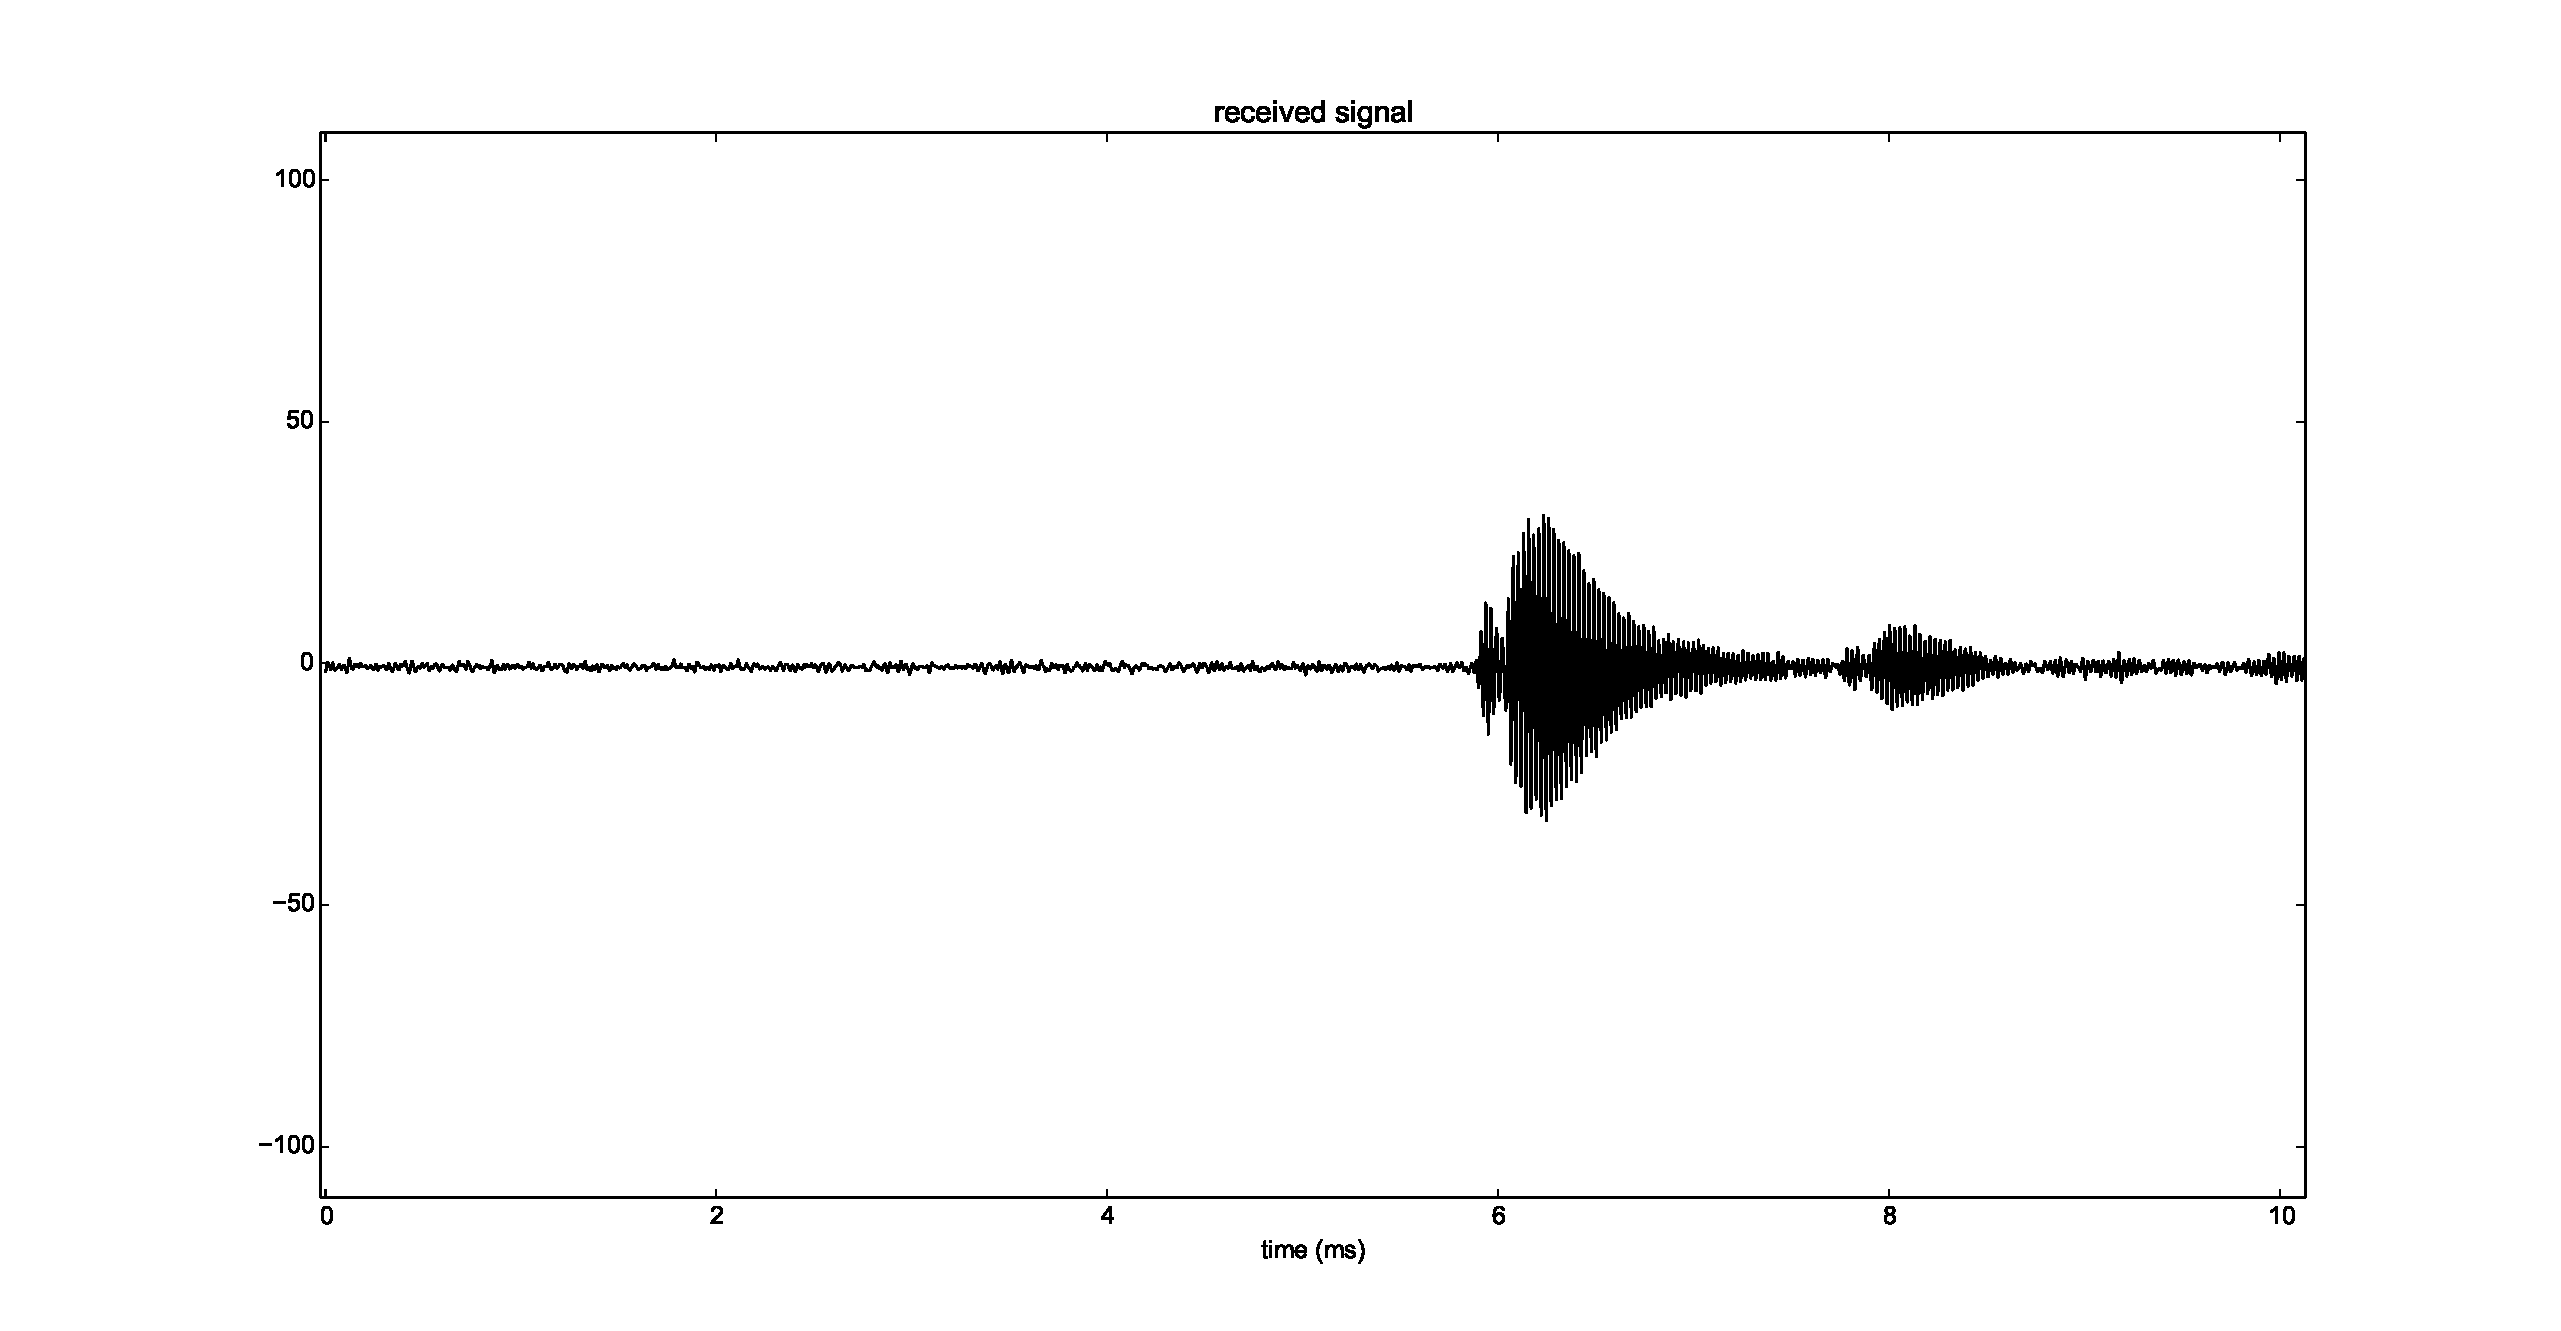
\includegraphics[width=1.0\textwidth, trim= 50mm 0mm 40mm 0mm,clip]{com_output_2m_1}
    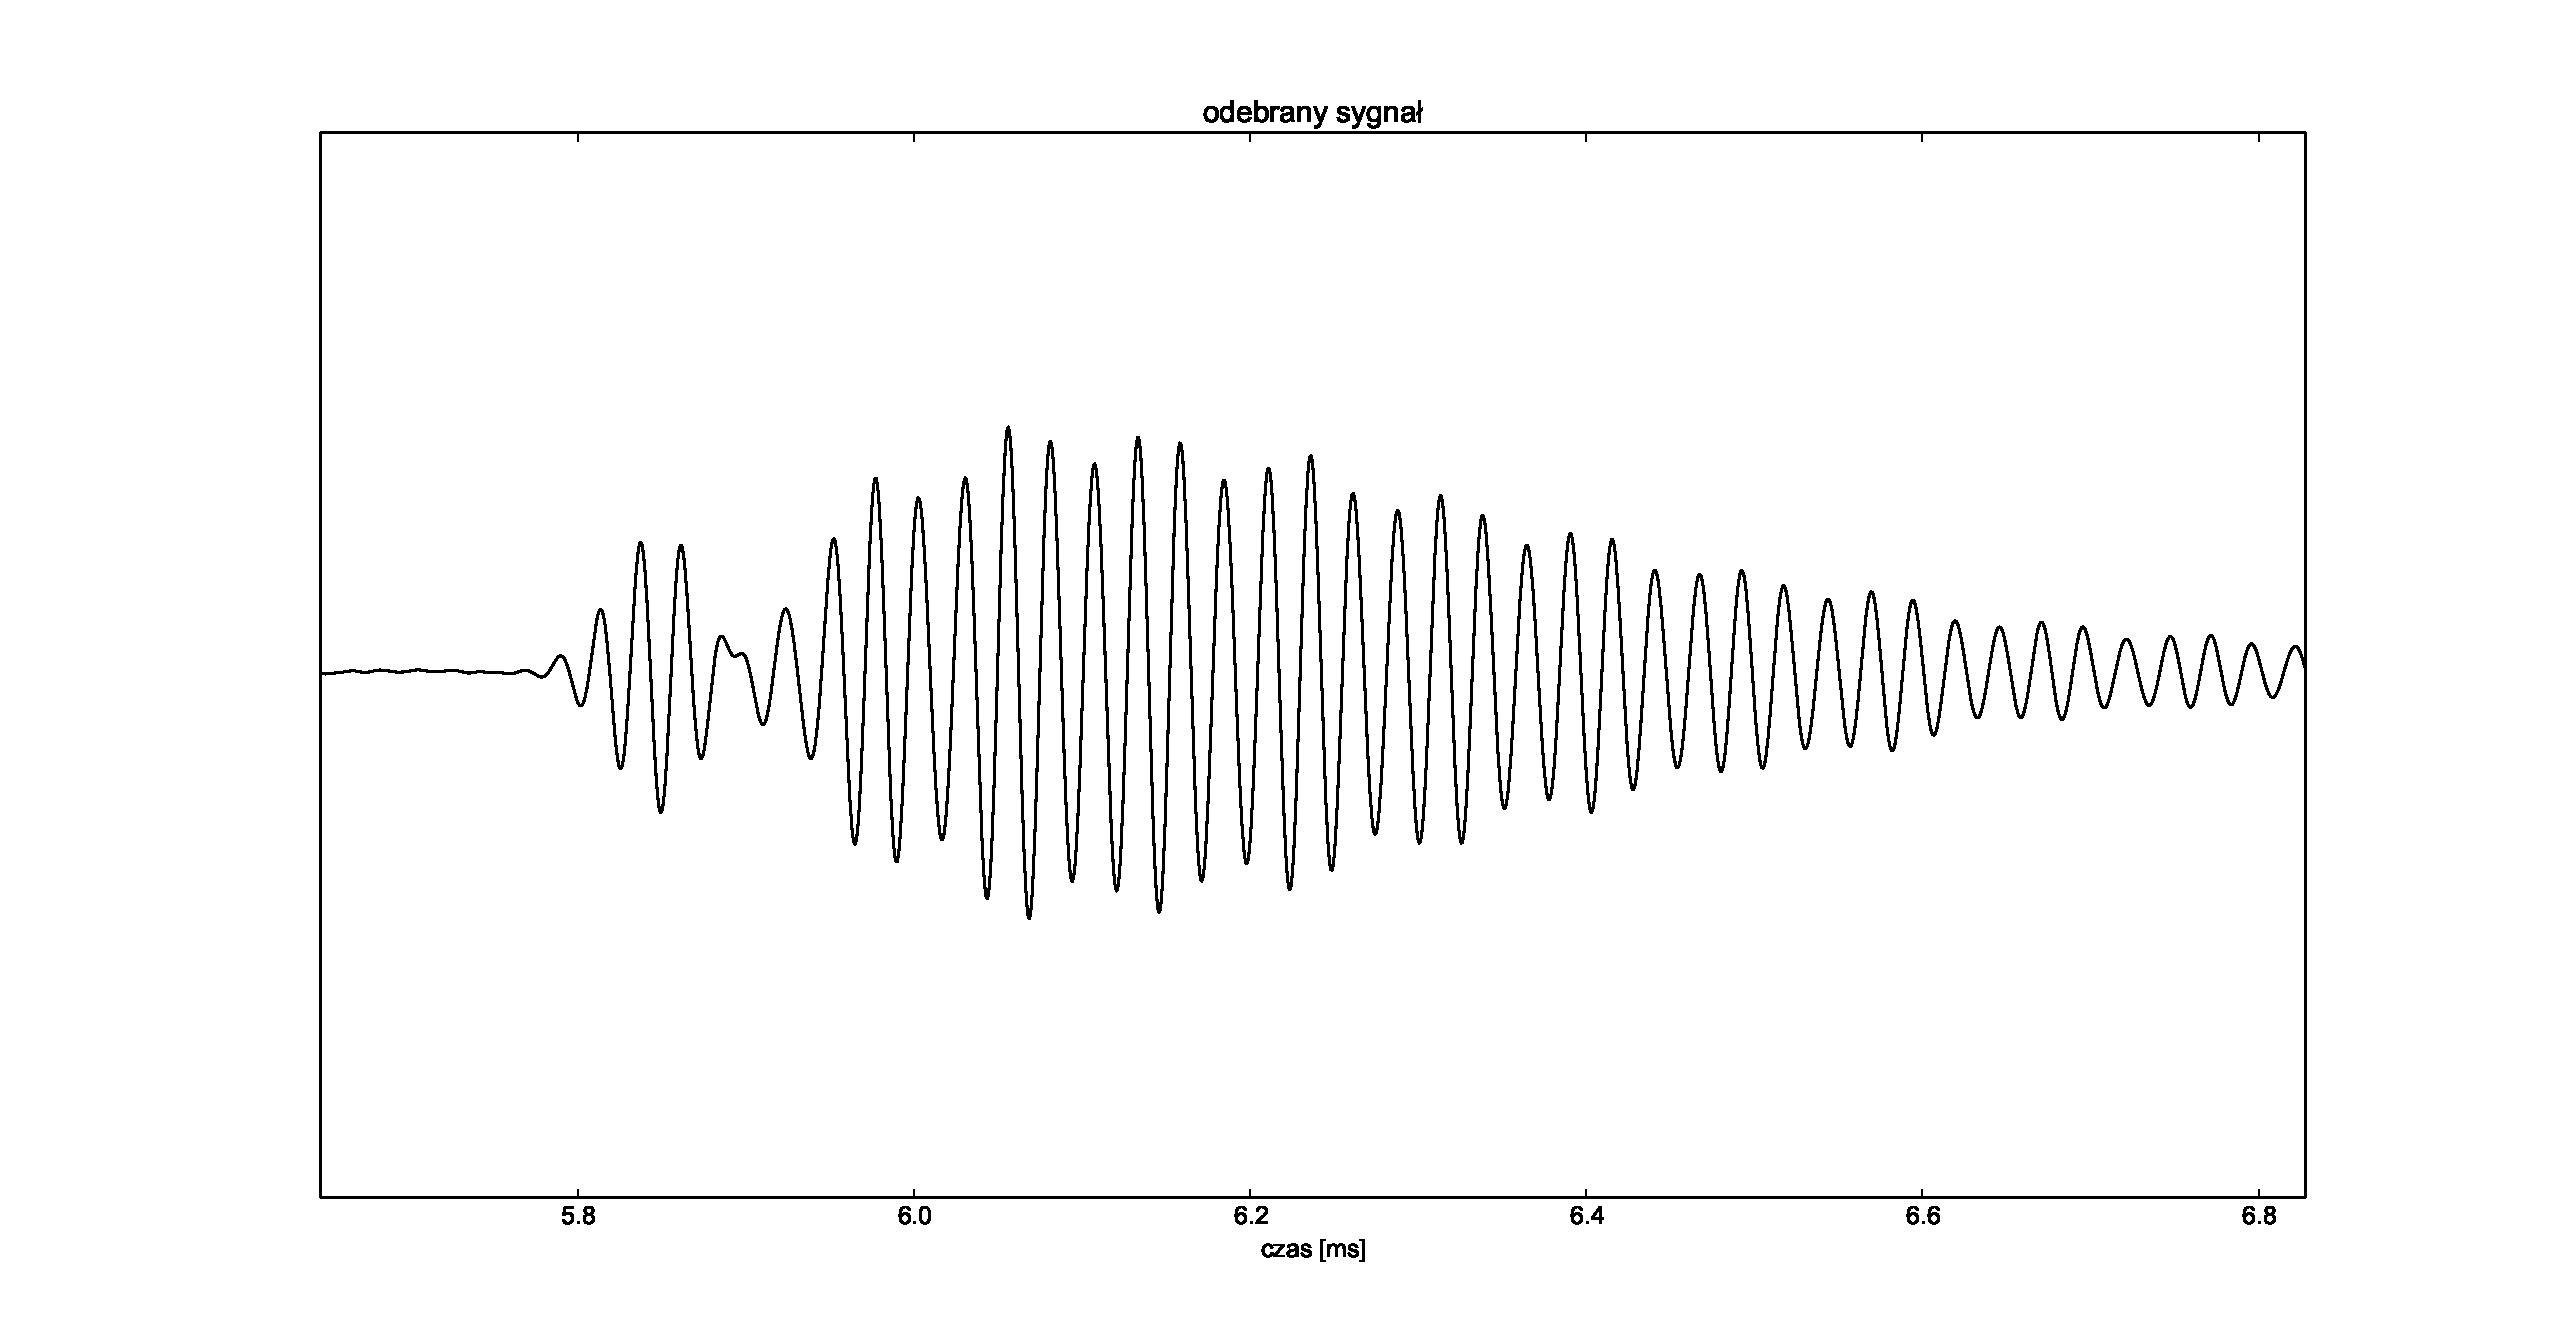
\includegraphics[width=1.0\textwidth, trim= 50mm 0mm 40mm 0mm,clip]{com_output_2m_2}
    \caption{Sygnał odebrany przez moduł \textit{com.py}. 
    Odległość między nadajnikiem a odbiornikiem wynosi \SI{2}{m}.
    Na górnym wykresie w przedziale \SI{6}{ms} i \SI{8}{ms} widać właściwy sygnał (poruszający się po linii prostej), a od \SI{8.5}{ms}
   widać sygnał odbity od podłogi. 
    Dolny wykres jest powiększeniem fragmentu górnego wykresu.}
    \label{fig:com_output_2m}
\end{figure}

\section{Wyznaczanie odległości, moduł \textit{find\_pattern.py}}

Moduł \textit{find\_pattern.py} odpowiada za obliczanie odległości pomiędzy czterema głośnikami i~trzema mikrofonami.
Wyznaczana jest ona przez wyszukanie w każdym z 12 odebranych sygnałów  położenia \textit{wzorca}, który 
odpowiada czołu nadanego sygnału (rysunek \ref{fig:com_output_2m}).
Wzorzec po raz pierwszy wprowadzana się podczas kalibracji, a  
podczas pracy urządzenia jest on ciągle aktualizowany.

Aby wyszukać wzorzec wewnątrz sygnału, korzysta się z  metody najmniejszego błędu średniokwadratowego.
Niech $w(t)$  dla $t = 0, ..., n-1$ będzie szukanym wzorcem, a $f(t)$ dla $t = 0, ..., m-1$ odebranym sygnałem.
Wtedy możemy znaleźć takie $a$, że błąd średniokwadratowy $E(t)$ pomiędzy $w$ i $a f |_{\{t, ..., t+n-1\}}$ jest minimalny.
Możemy to zapisać w postaci
\[
  E(t) = \min_{a \in R} \left\{ \sum_{i=0}^{n-1}  \left( w(i) - a f(t+i) \right) ^2 \right\}, \quad \text{dla } t = 0, ..., m-n.
\]
Po podniesieniu wyrażenia w nawiasie do kwadratu otrzymujemy
\[
  E(t) = \min_{a \in R} \left\{ \sum_{i=0}^{n-1}  \left( w^2(i) -2a w(i) f(t+i) + a^2 f^2(t+i) \right) \right\},
\]
\[
  E(t) = \min_{a \in R} \left\{ \sum_{i=0}^{n-1}  w^2(i) -2a \sum_{i=0}^{n-1}  w(i) f(t+i) + a^2 \sum_{i=0}^{n-1} f^2(t+i) \right\}.
\]
Aby wyliczyć $E(t)$, należy zminimalizować wyrażenie
\[
  y(a) = \sum_{i=0}^{n-1}  w^2(i) -2a \sum_{i=0}^{n-1}  w(i) f(t+i) + a^2 \sum_{i=0}^{n-1} f^2(t+i).
\]
Korzystając z faktu, że $y(a)$ jest funkcją kwadratową, możemy wyliczyć $a$ minimalizujące $y(a)$
\[
  a = \frac{ \sum\limits_{i=0}^{n-1}  w(i) f(t+i) }{ \sum\limits_{i=0}^{n-1} f^2(t+i) }.
\]
Ostatecznie dostajemy wzór na $E(t)$
\[
  E(t) = \sum_{i=0}^{n-1}  w^2(i)  - \frac {\left(\sum\limits_{i=0}^{n-1}  w(i) f(t+i) \right)^2 } { \sum\limits_{i=0}^{n-1} f^2(t+i)}.
\]

Zauważmy, że dzięki skalowaniu skalarem $a$  sygnału $f$, zamiast wzorca $w$,
otrzymane $E(t)$ nie zależy od siły odebranego sygnału. Ułatwia to porównanie błędów w dwóch różnych miejscach.
$E(t)$ zależy jednak od siły sygnału wzorcowego -- możemy się od niej uniezależnić, wyznaczając
błąd względny $e(t)$
\[
  e(t) = \frac{E(t)}{\sum\limits_{i=0}^{n-1}  w^2(i)}.
\]
Po podstawieniu $E(t)$ dostajemy
\[
  e(t) = 1 - \frac {\left(\sum\limits_{i=0}^{n-1}  w(i) f(t+i) \right)^2 } { \sum\limits_{i=0}^{n-1} f^2(t+i) \sum\limits_{i=0}^{n-1}  w^2(i)}.
\]
 
 Funkcję $e(t)$  można interpretować następująco:
 im mniejszy błąd $e(t)$, tym większe prawdopodobieństwo, że szukany wzorzec $w$ znajduje się na pozycji $t$ w 
 odebranym sygnale $f$. 

 Wynikiem obliczeń modułu \textit{find\_pattern.py} jest cała funkcja $e(t)$, na podstawie której moduł \textit{xyz.py}
 wyznacza pozycję i orientację nadajnika, uwzględniając przy tym 
 jego kształt (nadmiarowość danych), a także prawdopodobieństwo, że znaleziony wzorzec znajduje się w określonej pozycji.
 Rysunek \ref{fig:blad_korel} przedstawia wynik przetwarzania sygnału przez moduł \textit{find\_pattern.py}.

\begin{figure}[h]
    \centering
    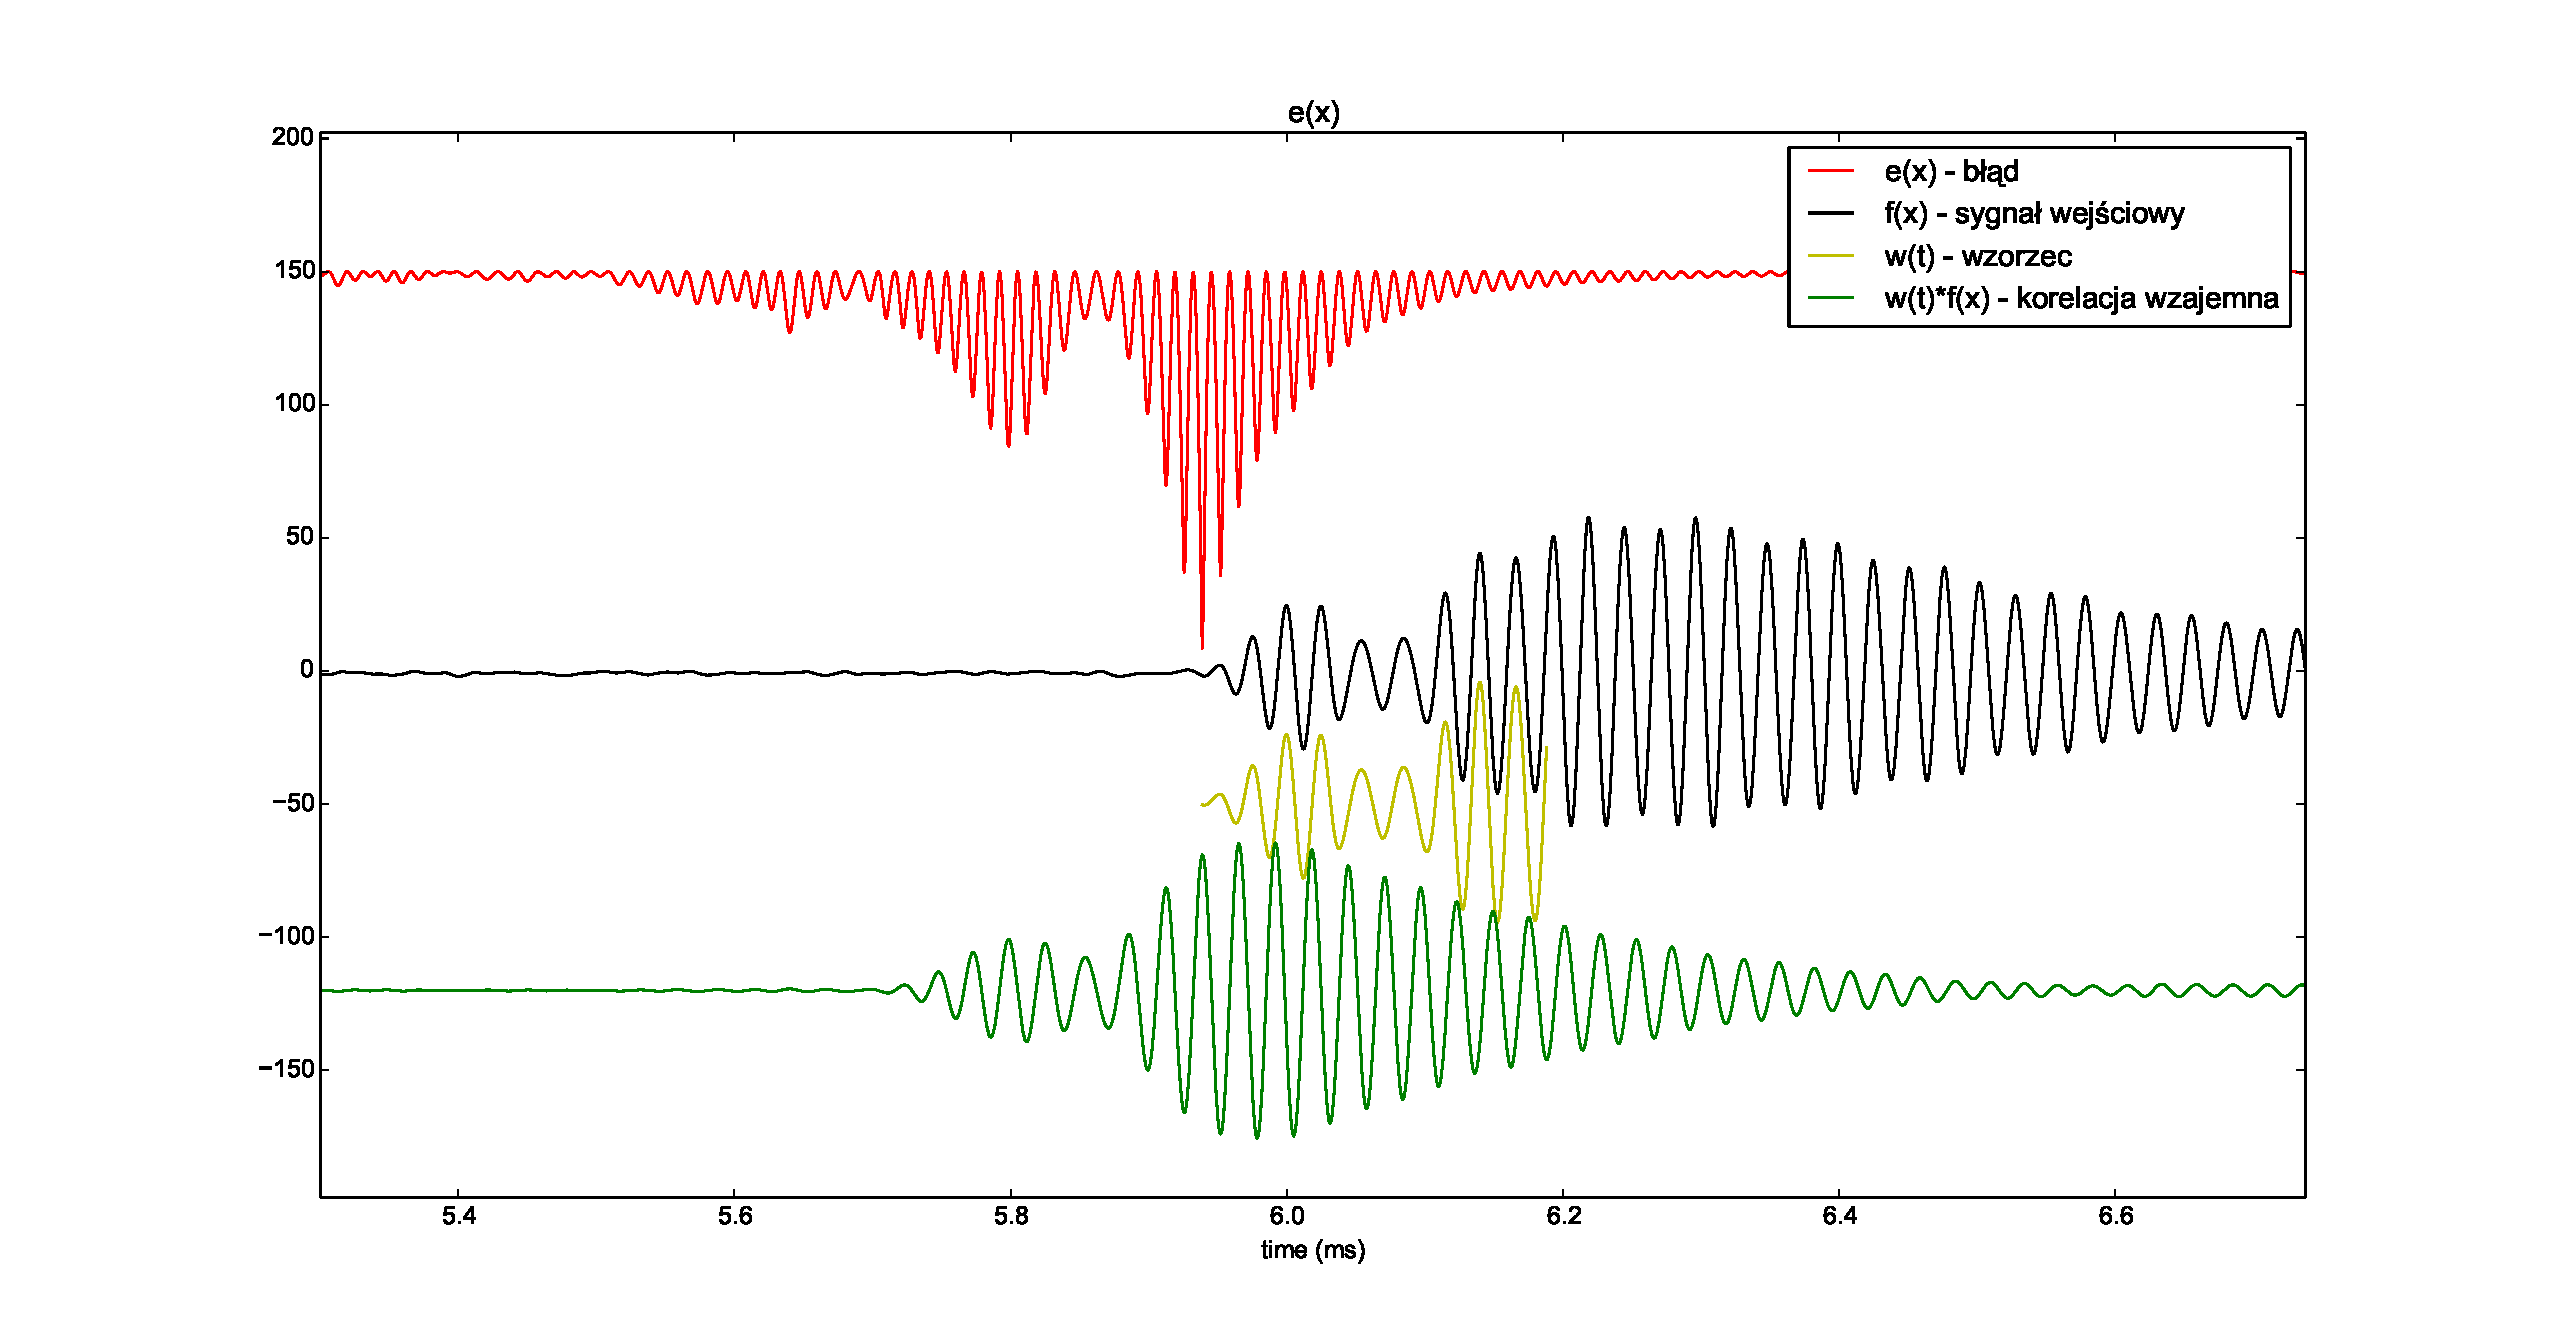
\includegraphics[width=1.0\textwidth, trim= 50mm 0mm 40mm 0mm,clip]{blad_korel}
    \caption{Sygnał przetworzony przez moduł \textit{find\_pattern.py}}
    \label{fig:blad_korel}
\end{figure}
 
 
 Wyliczenie zarówno $ \sum\limits_{i=0}^{n-1}  w^2(i) $,
jak i $\sum\limits_{i=0}^{n-1} f^2(t+i)$ wymaga jedynie liniowej liczby operacji, a 
 $\sum\limits_{i=0}^{n-1}  w(i) f(t+i) $ jest korelacją wzajemną funkcji $w(t)$ i $f(t)$, którą
 można wyliczyć w~czasie $k \log(k)$, korzystając z szybkiej transformacji Fouriera \cite{bib:FFT_correlation},
 gdzie $k = \max \{n,m\}$. Wyliczenie całej funkcji $e(t)$ wymaga zatem jedynie $k \log(k)$ operacji.

 
 Kolejne zadanie modułu \textit{find\_pattern.py} to uaktualnianie wzorca.
 Wraz ze zmianą kąta nachylenia nadajnika względem odbiornika zmienia się kształt odbieranego sygnału,
 dlatego jeśli badany sygnał $f(t)$ zawiera szukany wzorzec na pozycji $t_w$ 
 oraz spełnione są następujące warunki:
 \begin{itemize}
  \item moc sygnału $f(t_w), ..., f(t_w+n-1)$ jest wystarczająco duża, gdzie $n$ jest długością wzorca,
  \item błąd względny $e(t_w)$ pomiędzy sygnałem a wzorcem jest mały,
  \item moduł \textit{xyz.py} rozpozna otrzymaną pozycję $t_w$ jako pasującą do modelowanej rzeczywistości
 \end{itemize}
to moduł uaktualni wzorzec do wartości $f(t_w), ..., f(t_w+n-1)$.
 
 
\section{Wyznaczanie pozycji oraz orientacji przestrzennej, moduł \textit{xyz.py}}

Na ostatnim etapem obliczeń wyznaczane są współrzędne kartezjańskie czterech głośników umieszczonych na nadajniku.
Zajmuje się tym moduł \textit{xyz.py}, który dodatkowo zawiera prosty model rzeczywistości
rozpoznający niepoprawne dane o położeniu głośników.
Model zawiera informacje o wzajemnym położeniu czterech głośników w przestrzeni, co umożliwia wychwycenie 
zmiany geometrii nadajnika (niepoprawne odległości pomiędzy głośnikami).

Współrzędne głośników wyznacza się na podstawie dwunastu funkcji $e_{ij}(t)$ dla $i=1, ..., 4$ oraz $j=1, ..., 3$,
w których zawarta jest informacja o odległości pomiędzy głośnikiem $i$ oraz mikrofonem $j$.
Dla danej funkcji $e_{ij}(t)$ wyszukiwane są wszystkie wartości $t_m$, dla których funkcja osiąga minimum lokalne.
Następnie z $t_m$ wybierane są trzy punkty $t_{m_1}, t_{m_2}, t_{m_3}$, dla których wartość $e_{ij}(t_m)$ jest najmniejsza,
czyli spełniony został warunek:
\[ e_{ij}(t_{m_1}) \leq e_{ij}(t_{m_2}) \leq e_{ij}(t_{m_3}) \leq e_{ij}(t_m) \qquad \text{dla} \quad m \ne m_1,m_2,m_3. \]

Pozycje $t_{m_1}, t_{m_2}, t_{m_3}$  można interpretować jako trzy najbardziej prawdopodobne odległości 
pomiędzy głośnikiem a mikrofonem.

Do wyznaczenia położenia głośników w przestrzeni wykorzystywane są wszystkie możliwe kombinacje 
odległości $t_{m_1}, t_{m_2}, t_{m_3}$ dla każdej z dwunastu funkcji $e_{ij}$.
Daje to $12^3 = 1728$ możliwych lokalizacji głośników w przestrzeni. 
Każdą z nich sprawdza się z modelem (uzyskana geometria przestrzenna nadajnika musi zgadzać się z
modelem). Z tych, które pasują, wybierana jest lokalizacja o najmniejszym sumarycznym błędzie średniokwadratowym.

Ostatecznym wynikiem pracy modułu \textit{xyz.py} jest dwanaście wartości $t_{m_k}$ gdzie $k \in \{1,2,3\}$, 
dla każdej funkcji $e_{ij}$. Wartości te określają pozycję głośników w przestrzeni.

Dodatkowo wartości $t_{m_k}$ przekazywane są z powrotem do modułu \textit{find\_pattern.py} w celu aktualizacji wzorców.


\section{Kalibracja}

Po każdym uruchomieniu urządzenie wymagana kalibracji,
która polega na ustawieniu nadajnika w odległości 2 metrów od odbiornika,
uruchomieniu programu \textit{save-pattern.py} oraz zaznaczeniu w nim 12 obszarów  będącym czołem odebranego sygnału.
Obszary te wykorzystane zostaną jako wzorce podczas mierzenia odległości.
Program wyliczy także aktualną prędkość dźwięku, uwzględniając odległość nadajnika od odbiornika.

Rysunek \ref{fig:kalibracja_12x} przedstawia 12 sygnałów wraz z zaznaczonymi wzorcami.


 \begin{figure}[ht]
    \centering
    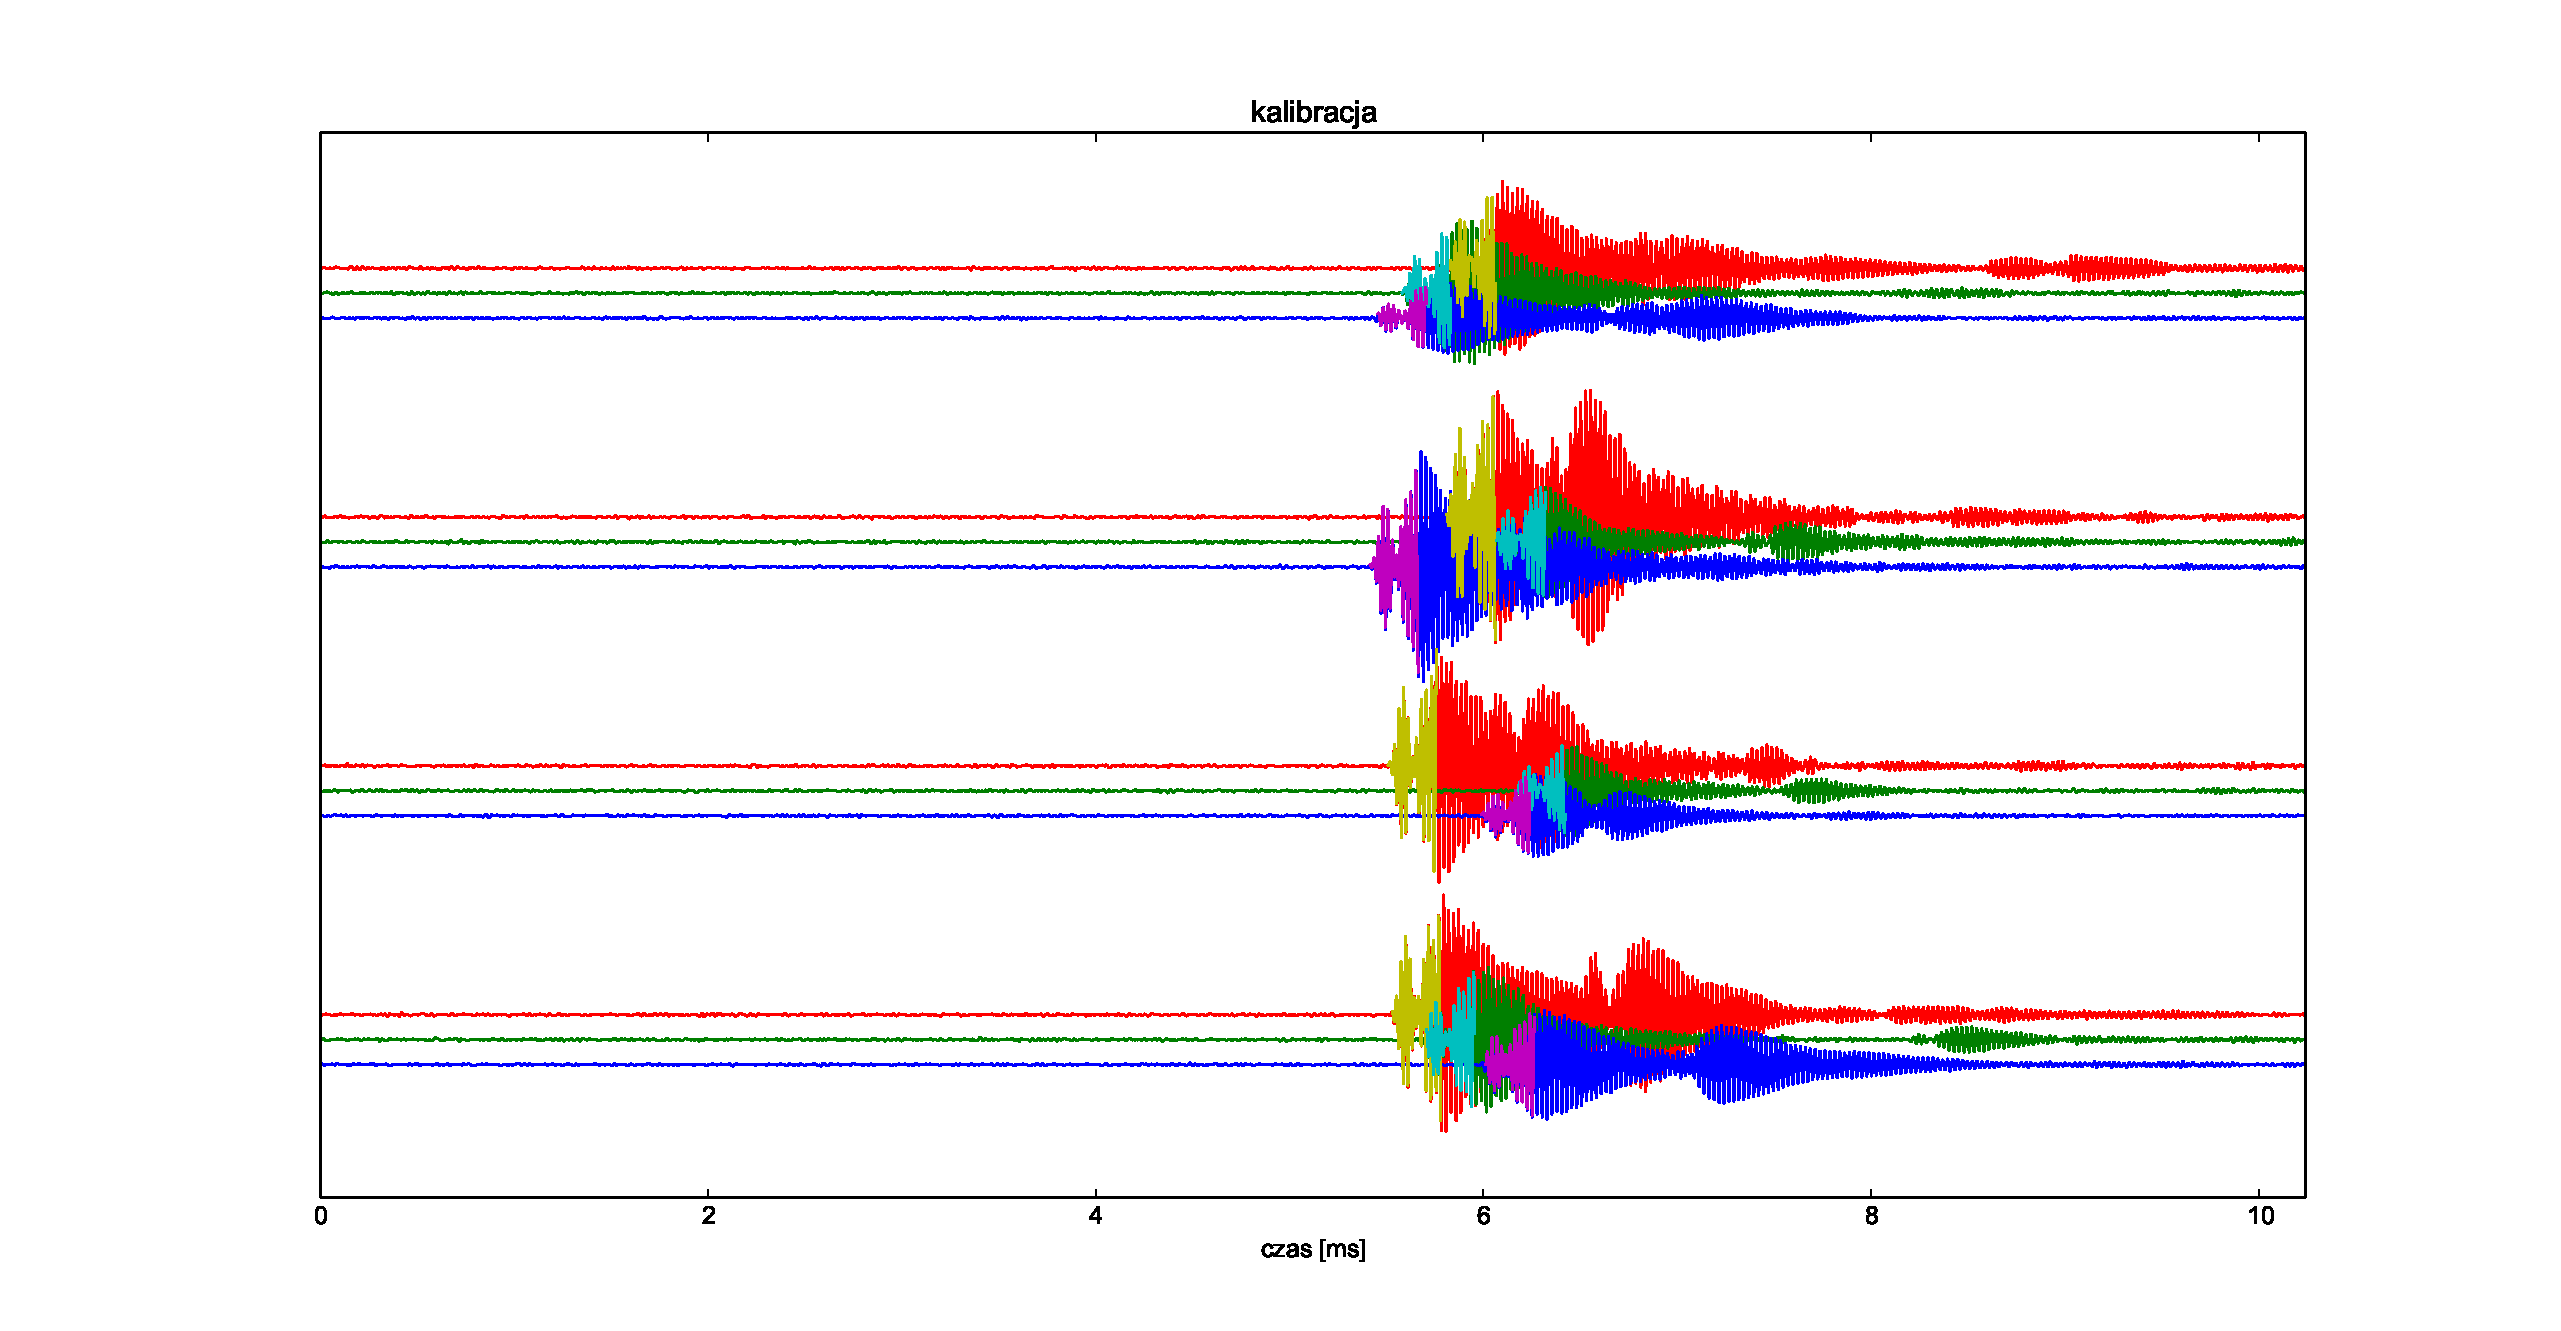
\includegraphics[width=1.0\textwidth, trim= 50mm 0mm 40mm 0mm,clip]{kalibracja_12x}
    \caption{Kalibracja, 12 sygnałów z zaznaczonymi wzorcami}
    \label{fig:kalibracja_12x}
\end{figure}

\newpage

\section{Obsługa programu \textit{scan.py}}

Do obsługi prototypu służy program \textit{scan.py}. Po jego uruchomieniu 
na monitorze wyświetlają się trzy okna: 
\begin{itemize}
 \item widok 3D prezentujący położenie nadajnika w przestrzeni -- w oknie widoczne są  
 4 punkty reprezentujące głośniki nadajnika oraz 3 prostopadłe względem siebie wektory określające 
jego orientację i położenie (rysunek \ref{fig:widok3d}),
 \item widok 2D, również przestawiający położenie nadajnika w przestrzeni --
 są to nałożone na siebie rzuty na płaszczyzny XY i XZ
 (rysunek \ref{fig:widok2d}),
 \item diagram informujący o mocy całego odebranego sygnału, mocy wzorca, mocy sygnału pasującego do wzorca 
 oraz błędzie pomiędzy wzorcem a odebranym sygnałem (rysunek \ref{fig:power}).
\end{itemize}

Wszelkie zmiany położenia nadajnika automatycznie odświeżają wszystkie widoki. 
Podczas uruchamiania programu aktualne położenie nadajnika przyjmowane 
jest jako początek układu współrzędnych.
Jeśli któryś z głośników straci widoczność z mikrofonami, obraz przestaje się odświeżać, a informacja, dlaczego tak
się dzieje, widoczna jest w oknie przedstawiającym moc sygnału.


\rysunekHT{3d}{Widok 3D}{\label{fig:widok3d}}
\rysunekHT{2d}{Widok 2D}{\label{fig:widok2d}}
\rysunekHT{power}{Diagram informujący o mocy całego odebranego sygnału, mocy wzorca, mocy sygnału pasującego do wzorca 
 oraz błędzie pomiędzy wzorcem a odebranym sygnałem}{\label{fig:power}}

